% ============================================================
% 高考满分突破9 — 复数与欧拉公式
% 编译命令：xelatex -interaction=nonstopmode 高考满分突破9_复数与欧拉公式.tex
% ============================================================
\documentclass[12pt, a4paper]{ctexart}
\usepackage[margin=2.2cm]{geometry}
\usepackage{amsmath, amssymb}
\usepackage{enumitem}
\usepackage{tcolorbox}
\usepackage{booktabs}
\usepackage{array}
\usepackage{fancyhdr}
\usepackage{xcolor}
\usepackage{tikz}
\usepackage{hyperref}
\usepackage{graphicx}
\usepackage{multirow}
\usepackage{pgfplots}
\pgfplotsset{compat=1.18}

% 颜色定义
\definecolor{mainblue}{RGB}{41, 98, 168}
\definecolor{lightblue}{RGB}{230, 240, 255}
\definecolor{tipgreen}{RGB}{34, 139, 87}
\definecolor{lightgreen}{RGB}{235, 250, 240}
\definecolor{warnred}{RGB}{200, 50, 50}
\definecolor{lightred}{RGB}{255, 240, 240}
\definecolor{examorange}{RGB}{210, 120, 20}
\definecolor{lightorange}{RGB}{255, 248, 235}
\definecolor{apppurple}{RGB}{120, 60, 170}
\definecolor{lightpurple}{RGB}{245, 238, 255}

% 页眉页脚
\pagestyle{fancy}
\fancyhf{}
\fancyhead[L]{\small\textcolor{mainblue}{\textbf{高考满分突破 · 复数与欧拉公式}}}
\fancyhead[R]{\small\textcolor{mainblue}{讲义09}}
\fancyfoot[C]{\small —\ \thepage\ —}
\renewcommand{\headrulewidth}{0.6pt}
\renewcommand{\headrule}{\hbox to\headwidth{\color{mainblue}\leaders\hrule height \headrulewidth\hfill}}
\renewcommand{\footrulewidth}{0pt}

% tcolorbox 样式
\newtcolorbox{knowledgebox}[1][]{%
  colback=lightblue, colframe=mainblue,
  fonttitle=\bfseries\large, title=#1,
  arc=3mm, boxrule=0.8pt,
  left=8pt, right=8pt, top=6pt, bottom=6pt
}

\newtcolorbox{tipbox}[1][]{%
  colback=lightgreen, colframe=tipgreen,
  fonttitle=\bfseries, title=#1,
  arc=2mm, boxrule=0.6pt,
  left=6pt, right=6pt, top=4pt, bottom=4pt
}

\newtcolorbox{warnbox}[1][]{%
  colback=lightred, colframe=warnred,
  fonttitle=\bfseries, title=#1,
  arc=2mm, boxrule=0.6pt,
  left=6pt, right=6pt, top=4pt, bottom=4pt
}

\newtcolorbox{examplebox}[1][]{%
  colback=lightorange, colframe=examorange,
  fonttitle=\bfseries, title=#1,
  arc=3mm, boxrule=0.8pt,
  left=8pt, right=8pt, top=6pt, bottom=6pt
}

\newtcolorbox{appbox}[1][]{%
  colback=lightpurple, colframe=apppurple,
  fonttitle=\bfseries, title=#1,
  arc=3mm, boxrule=0.8pt,
  left=8pt, right=8pt, top=6pt, bottom=6pt
}

\setCJKmainfont{Hiragino Sans GB}
\setCJKsansfont{Heiti SC}

\begin{document}

% ============ 标题页 ============
\begin{center}
{\Huge\bfseries\textcolor{mainblue}{高考数学满分突破}}\\[6pt]
{\LARGE\bfseries\textcolor{mainblue}{复数与欧拉公式}}\\[12pt]
\rule{0.6\textwidth}{1pt}\\[8pt]
{\normalsize 适用：高三冲刺\quad |\quad 课时：2课时}
\end{center}
\vspace{10pt}

% ============================================================
%  第一部分：知识点讲解
% ============================================================
\section*{\textcolor{mainblue}{一、知识点讲解}}

% —— 1.1 欧拉公式 ——
\subsection*{1.1\quad 欧拉公式 $e^{i\theta}$}

\begin{knowledgebox}[欧拉公式]
对任意实数 $\theta$，有
\[
  \boxed{e^{i\theta} = \cos\theta + i\sin\theta}
\]
当 $\theta = \pi$ 时，得到数学中最优美的等式——欧拉恒等式：
\[
  e^{i\pi} + 1 = 0
\]
它将五个最重要的数学常数 $e,\,i,\,\pi,\,1,\,0$ 统一在一个等式中。
\end{knowledgebox}

\begin{tipbox}[几何直观]
将 $e^{i\theta}$ 看作复平面上的点，它恰好在单位圆上，与实轴夹角为 $\theta$（弧度）。当 $\theta$ 从 $0$ 增大到 $2\pi$ 时，$e^{i\theta}$ 沿单位圆逆时针旋转一周。
\begin{center}
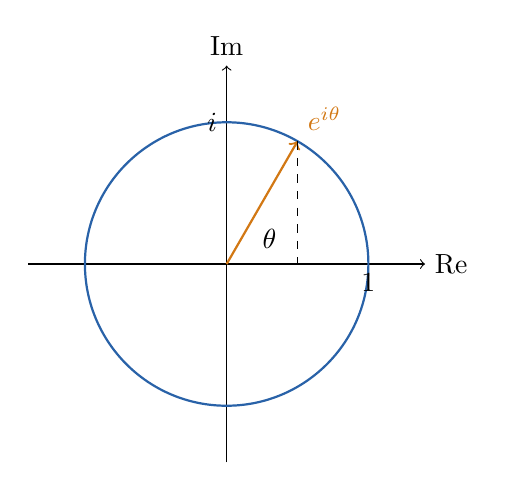
\begin{tikzpicture}[scale=1.8]
  \draw[->] (-1.4,0)--(1.4,0) node[right]{$\text{Re}$};
  \draw[->] (0,-1.4)--(0,1.4) node[above]{$\text{Im}$};
  \draw[thick, mainblue] (0,0) circle(1);
  \draw[thick, ->, examorange] (0,0)--(60:1) node[above right]{$e^{i\theta}$};
  \draw[dashed] (60:1)--(60:1 |- 0,0);
  \node at (30:0.35) {$\theta$};
  \node[below] at (1,0) {$1$};
  \node[left] at (0,1) {$i$};
\end{tikzpicture}
\end{center}
\end{tipbox}

\begin{knowledgebox}[指数运算法则]
对实数 $\alpha,\,\beta$，欧拉公式满足：
\begin{enumerate}[label=(\arabic*)]
  \item $e^{i\alpha}\cdot e^{i\beta} = e^{i(\alpha+\beta)}$；
  \item $\left(e^{i\theta}\right)^n = e^{in\theta}$（棣莫弗公式）；
  \item $e^{-i\theta} = \cos\theta - i\sin\theta$。
\end{enumerate}
由此可得：
\[
  \cos\theta = \frac{e^{i\theta}+e^{-i\theta}}{2}, \qquad
  \sin\theta = \frac{e^{i\theta}-e^{-i\theta}}{2i}
\]
\end{knowledgebox}

% —— 1.2 用复数证三角恒等式 ——
\subsection*{1.2\quad 用复数证明三角恒等式}

\begin{knowledgebox}[核心思路]
利用 $e^{i\theta}=\cos\theta+i\sin\theta$，将三角问题转化为复数指数运算，再取实部或虚部，即可推导三角恒等式。
\end{knowledgebox}

\begin{tipbox}[常用恒等式的复数推导]
\textbf{（1）两角和公式：}
\[
  e^{i(\alpha+\beta)} = e^{i\alpha}\cdot e^{i\beta}
  = (\cos\alpha+i\sin\alpha)(\cos\beta+i\sin\beta)
\]
展开右边，比较实部和虚部：
\[
  \cos(\alpha+\beta) = \cos\alpha\cos\beta - \sin\alpha\sin\beta
\]
\[
  \sin(\alpha+\beta) = \sin\alpha\cos\beta + \cos\alpha\sin\beta
\]

\textbf{（2）倍角公式：}
令 $\alpha=\beta=\theta$，即得
\[
  \cos 2\theta = \cos^2\theta - \sin^2\theta, \qquad
  \sin 2\theta = 2\sin\theta\cos\theta
\]

\textbf{（3）三倍角公式（棣莫弗）：}
由 $(\cos\theta+i\sin\theta)^3 = \cos 3\theta + i\sin 3\theta$，展开左边取实部/虚部：
\[
  \cos 3\theta = 4\cos^3\theta - 3\cos\theta, \qquad
  \sin 3\theta = 3\sin\theta - 4\sin^3\theta
\]
\end{tipbox}

% —— 1.3 复数与旋转对称 ——
\subsection*{1.3\quad 复数与旋转对称}

\begin{knowledgebox}[复数乘法的几何意义]
设 $z_1 = r_1 e^{i\theta_1}$，$z_2 = r_2 e^{i\theta_2}$，则
\[
  z_1 \cdot z_2 = r_1 r_2\, e^{i(\theta_1+\theta_2)}
\]
即：\textbf{模相乘，辐角相加}。因此乘以 $e^{i\theta}$ 相当于将向量逆时针旋转 $\theta$。
\end{knowledgebox}

\begin{knowledgebox}[单位根与正多边形]
方程 $z^n = 1$ 的 $n$ 个根为
\[
  \omega_k = e^{\frac{2\pi i k}{n}},\qquad k=0,1,2,\ldots,n-1
\]
它们在复平面上构成正 $n$ 边形的顶点，称为 \textbf{$n$ 次单位根}。特别地，$\omega = e^{\frac{2\pi i}{n}}$ 为\textbf{本原 $n$ 次单位根}，满足 $\omega^n=1$，且
\[
  1+\omega+\omega^2+\cdots+\omega^{n-1}=0
\]
\end{knowledgebox}

\begin{warnbox}[易错提醒]
\begin{enumerate}[label=(\arabic*)]
  \item $(z_1 z_2)^n = z_1^n z_2^n$ 只在 $z_1,z_2$ 为复数且 $n$ 为整数时成立；当涉及开方时需注意多值性。
  \item $\arg(z_1 z_2) = \arg z_1 + \arg z_2 + 2k\pi$（$k\in\mathbb{Z}$），辐角相加需要 $\bmod\,2\pi$。
  \item 高考中复数题多在选择填空，计算务必准确区分实部和虚部。
\end{enumerate}
\end{warnbox}

% —— 1.4 高考三角函数复数解法 ——
\subsection*{1.4\quad 高考三角函数的复数解法}

\begin{knowledgebox}[复数方法在高考中的应用策略]
虽然高考不要求掌握欧拉公式，但复数工具可以\textbf{快速验证}和\textbf{简化计算}：
\begin{enumerate}[label=(\arabic*)]
  \item 求 $\cos^n\theta$ 或 $\sin^n\theta$ 的展开：用 $\cos\theta = \frac{e^{i\theta}+e^{-i\theta}}{2}$ 二项式展开后取实部。
  \item 求形如 $\displaystyle\sum_{k=0}^{n-1}\cos(a+kd)$ 的和：转化为等比数列 $\displaystyle\sum e^{i(a+kd)}$ 求和后取实部。
  \item 证明三角恒等式：转化为复数等式后展开比较。
  \item 利用 $1$ 的 $n$ 次单位根求和为零的性质，快速计算含有 $\cos\frac{2k\pi}{n}$、$\sin\frac{2k\pi}{n}$ 的表达式。
\end{enumerate}
\end{knowledgebox}

% ============================================================
%  第二部分：例题精讲
% ============================================================
\section*{\textcolor{examorange}{二、例题精讲}}

\begin{examplebox}[【例题1】欧拉公式基本运算]
计算 $e^{i\pi/4}\cdot e^{i\pi/6}$，并将其写为 $a+bi$ 的形式。
\end{examplebox}

\textbf{解：}
\[
  e^{i\pi/4}\cdot e^{i\pi/6} = e^{i(\pi/4+\pi/6)} = e^{i\cdot 5\pi/12}
\]
\[
  = \cos\frac{5\pi}{12}+i\sin\frac{5\pi}{12}
\]
由半角公式：$\cos\frac{5\pi}{12}=\cos 75°=\frac{\sqrt{6}-\sqrt{2}}{4}$，$\sin\frac{5\pi}{12}=\sin 75°=\frac{\sqrt{6}+\sqrt{2}}{4}$。
\[
  \boxed{\dfrac{\sqrt{6}-\sqrt{2}}{4}+\dfrac{\sqrt{6}+\sqrt{2}}{4}\,i}
\]

\begin{examplebox}[【例题2】棣莫弗公式求 $\cos 3\theta$]
利用棣莫弗公式推导 $\cos 3\theta = 4\cos^3\theta - 3\cos\theta$。
\end{examplebox}

\textbf{解：}
由棣莫弗公式，$(\cos\theta+i\sin\theta)^3 = \cos 3\theta+i\sin 3\theta$。

展开左边：
\[
  (\cos\theta+i\sin\theta)^3 = \cos^3\theta + 3i\cos^2\theta\sin\theta - 3\cos\theta\sin^2\theta - i\sin^3\theta
\]
取实部：
\[
  \cos 3\theta = \cos^3\theta - 3\cos\theta\sin^2\theta
  = \cos^3\theta - 3\cos\theta(1-\cos^2\theta)
  = 4\cos^3\theta - 3\cos\theta \qquad\blacksquare
\]

\begin{examplebox}[【例题3】用复数求三角级数和]
求 $\displaystyle S = \sum_{k=0}^{n-1}\cos\frac{2k\pi}{n}$ 的值（$n\geq 2$）。
\end{examplebox}

\textbf{解：}
令 $\omega = e^{2\pi i/n}$，则
\[
  \sum_{k=0}^{n-1}e^{2\pi ik/n} = \sum_{k=0}^{n-1}\omega^k
\]
这是首项为 $1$、公比为 $\omega\neq 1$ 的等比数列，其和为
\[
  \frac{1-\omega^n}{1-\omega} = \frac{1-1}{1-\omega} = 0
\]
取实部：$\displaystyle S = \operatorname{Re}\left(\sum_{k=0}^{n-1}\omega^k\right) = \boxed{0}$。

\begin{tipbox}[方法总结]
此类三角级数求和问题，用复数方法极为简洁：将 $\cos$ 换成 $e^{i\theta}$，利用单位根等比求和，再取实部即可。
\end{tipbox}

\begin{examplebox}[【例题4】复数的模与辐角]
设 $z = \dfrac{(1+i)^4}{(1-i)^3}$，求 $|z|$ 和 $\arg z$。
\end{examplebox}

\textbf{解：}
先将 $1+i$ 和 $1-i$ 化为指数形式：
\[
  1+i = \sqrt{2}\,e^{i\pi/4}, \qquad 1-i = \sqrt{2}\,e^{-i\pi/4}
\]
因此
\[
  z = \frac{(\sqrt{2}\,e^{i\pi/4})^4}{(\sqrt{2}\,e^{-i\pi/4})^3}
  = \frac{4\,e^{i\pi}}{2\sqrt{2}\,e^{-3i\pi/4}}
  = \sqrt{2}\,e^{i(\pi+3\pi/4)}
  = \sqrt{2}\,e^{i\cdot 7\pi/4}
\]
所以 $|z|=\boxed{\sqrt{2}}$，$\arg z = \boxed{\dfrac{7\pi}{4}}$（即 $-45°$）。

\begin{examplebox}[【例题5】单位根求值]
设 $\omega = e^{2\pi i/5}$，求 $1+\omega+\omega^2+\omega^3+\omega^4$ 的值，并由此计算 $\cos\dfrac{2\pi}{5}+\cos\dfrac{4\pi}{5}+\cos\dfrac{6\pi}{5}+\cos\dfrac{8\pi}{5}$。
\end{examplebox}

\textbf{解：}
$\omega$ 是 $z^5=1$ 的本原根，故 $1+\omega+\omega^2+\omega^3+\omega^4=0$。

取实部：
\[
  1+\cos\frac{2\pi}{5}+\cos\frac{4\pi}{5}+\cos\frac{6\pi}{5}+\cos\frac{8\pi}{5} = 0
\]
所以
\[
  \cos\frac{2\pi}{5}+\cos\frac{4\pi}{5}+\cos\frac{6\pi}{5}+\cos\frac{8\pi}{5} = \boxed{-1}
\]

\begin{examplebox}[【例题6】用复数推导积化和差]
利用欧拉公式证明：$\cos\alpha\cos\beta = \dfrac{1}{2}[\cos(\alpha-\beta)+\cos(\alpha+\beta)]$。
\end{examplebox}

\textbf{解：}
由 $\cos\theta = \frac{e^{i\theta}+e^{-i\theta}}{2}$：
\begin{align*}
  \cos\alpha\cos\beta &= \frac{e^{i\alpha}+e^{-i\alpha}}{2}\cdot\frac{e^{i\beta}+e^{-i\beta}}{2} \\
  &= \frac{1}{4}\left(e^{i(\alpha+\beta)}+e^{i(\alpha-\beta)}+e^{-i(\alpha-\beta)}+e^{-i(\alpha+\beta)}\right) \\
  &= \frac{1}{2}\left[\frac{e^{i(\alpha+\beta)}+e^{-i(\alpha+\beta)}}{2}+\frac{e^{i(\alpha-\beta)}+e^{-i(\alpha-\beta)}}{2}\right] \\
  &= \frac{1}{2}[\cos(\alpha+\beta)+\cos(\alpha-\beta)] \qquad\blacksquare
\end{align*}

\begin{examplebox}[【例题7】复数旋转应用]
在复平面上，将点 $z=3+4i$ 绕原点逆时针旋转 $90°$，求旋转后的点对应的复数。
\end{examplebox}

\textbf{解：}
逆时针旋转 $90°$ 等价于乘以 $e^{i\pi/2}=i$：
\[
  z' = (3+4i)\cdot i = 3i+4i^2 = -4+3i
\]
旋转后的复数为 $\boxed{-4+3i}$。

\begin{tipbox}[旋转公式]
绕原点逆时针旋转 $\theta$：$z\mapsto z\cdot e^{i\theta}$。\\
绕点 $z_0$ 旋转：$z\mapsto (z-z_0)e^{i\theta}+z_0$。
\end{tipbox}

\begin{examplebox}[【例题8】复数与实系数方程]
已知实系数方程 $x^3-1=0$，用复数方法求其全部根，并验证根的对称性。
\end{examplebox}

\textbf{解：}
$x^3=1$ 的根为 $x=e^{2\pi ik/3}$，$k=0,1,2$，即
\[
  x_1 = 1,\qquad x_2 = e^{2\pi i/3} = -\frac{1}{2}+\frac{\sqrt{3}}{2}\,i, \qquad x_3 = e^{4\pi i/3} = -\frac{1}{2}-\frac{\sqrt{3}}{2}\,i
\]
验证：$x_1+x_2+x_3=0$（韦达定理，三次方程无 $x^2$ 项），$x_2$ 与 $x_3$ 互为共轭。$\blacksquare$

\begin{examplebox}[【例题9】$\cos^n\theta$ 的展开]
利用复数方法将 $\cos^4\theta$ 表示为 $\cos k\theta$（$k=0,2,4$）的线性组合。
\end{examplebox}

\textbf{解：}
\[
  \cos^4\theta = \left(\frac{e^{i\theta}+e^{-i\theta}}{2}\right)^4
  = \frac{1}{16}(e^{i\theta}+e^{-i\theta})^4
\]
展开：
\[
  (e^{i\theta}+e^{-i\theta})^4 = e^{4i\theta}+4e^{2i\theta}+6+4e^{-2i\theta}+e^{-4i\theta}
\]
所以
\[
  \cos^4\theta = \frac{1}{16}\left[2\cos 4\theta + 8\cos 2\theta + 6\right]
  = \boxed{\frac{1}{8}\cos 4\theta + \frac{1}{2}\cos 2\theta + \frac{3}{8}}
\]

\begin{examplebox}[【例题10】综合——复数与三角恒等式]
证明恒等式：$\displaystyle\prod_{k=1}^{n-1}\sin\frac{k\pi}{n} = \frac{n}{2^{n-1}}$。
\end{examplebox}

\textbf{解：}
考虑 $z^n-1 = \displaystyle\prod_{k=0}^{n-1}(z-\omega_k)$，其中 $\omega_k=e^{2\pi ik/n}$。

令 $z=1$：
\[
  \lim_{z\to 1}\frac{z^n-1}{z-1} = n = \prod_{k=1}^{n-1}(1-\omega_k)
\]
取模：
\[
  |1-\omega_k| = |1-e^{2\pi ik/n}| = 2\sin\frac{k\pi}{n}
\]
（利用 $|1-e^{i\alpha}|=2|\sin(\alpha/2)|$）。

所以
\[
  n = \prod_{k=1}^{n-1}2\sin\frac{k\pi}{n} = 2^{n-1}\prod_{k=1}^{n-1}\sin\frac{k\pi}{n}
\]
\[
  \prod_{k=1}^{n-1}\sin\frac{k\pi}{n} = \frac{n}{2^{n-1}} \qquad\blacksquare
\]

% ============================================================
%  第三部分：应用题
% ============================================================
\section*{\textcolor{apppurple}{三、应用题}}

\begin{appbox}[【应用1】信号处理中的复数]
在信号处理中，一个正弦信号可以表示为复指数形式。已知信号 $s(t) = 3\cos(2\pi t + \pi/3)$，将其写为复指数形式 $s(t) = \operatorname{Re}[Ae^{i(\omega t + \varphi)}]$，并确定振幅 $A$、角频率 $\omega$ 和初相位 $\varphi$。
\end{appbox}

\textbf{解：}
$s(t) = \operatorname{Re}[3e^{i(2\pi t+\pi/3)}]$，所以 $A=3$，$\omega=2\pi$，$\varphi=\pi/3$。

若两个信号 $s_1(t)=A_1\cos(\omega t+\varphi_1)$ 和 $s_2(t)=A_2\cos(\omega t+\varphi_2)$ 叠加，可用复数相加后再取实部：
\[
  A_1 e^{i\varphi_1}+A_2 e^{i\varphi_2} = Re^{i\Phi}
\]
合成信号的振幅 $R$ 和相位 $\Phi$ 可直接由复数运算得到。

\begin{appbox}[【应用2】正多边形的顶点坐标]
一个正六边形的中心在原点，一个顶点在 $(2,0)$。求其余五个顶点的坐标。
\end{appbox}

\textbf{解：}
正六边形的顶点为 $z_k = 2e^{2\pi ik/6} = 2e^{i\pi k/3}$，$k=0,1,\ldots,5$。

\begin{center}
\begin{tabular}{cccccc}
\toprule
$k$ & $0$ & $1$ & $2$ & $3$ & $4$ \\
\midrule
坐标 & $(2,0)$ & $(1,\sqrt{3})$ & $(-1,\sqrt{3})$ & $(-2,0)$ & $(-1,-\sqrt{3})$ \\
\bottomrule
\end{tabular}
\end{center}
（$k=5$ 对应 $(1,-\sqrt{3})$。）

\begin{appbox}[【应用3】交流电路中的复数阻抗]
在交流电路中，电阻 $R$、电感 $L$、电容 $C$ 的阻抗分别为 $Z_R=R$、$Z_L=i\omega L$、$Z_C=\dfrac{1}{i\omega C}$。一个串联 RLC 电路中 $R=3\,\Omega$，$\omega L=4\,\Omega$，$\dfrac{1}{\omega C}=2\,\Omega$，求总阻抗 $Z$ 及其模 $|Z|$。
\end{appbox}

\textbf{解：}
\[
  Z = Z_R + Z_L + Z_C = 3 + 4i + \frac{1}{i\omega C}
\]
注意 $\frac{1}{i\omega C} = \frac{-i}{\omega C} = -2i$，所以
\[
  Z = 3 + 4i - 2i = 3 + 2i
\]
\[
  |Z| = \sqrt{3^2+2^2} = \boxed{\sqrt{13}\approx 3.61\,\Omega}
\]

% ============================================================
%  第四部分：课堂练习
% ============================================================
\section*{\textcolor{tipgreen}{四、课堂练习}}

\begin{enumerate}
  \item 计算 $e^{i\pi/3}\cdot e^{i\pi/4}$，并写为 $a+bi$ 的形式。

  \item 利用棣莫弗公式求 $\sin 3\theta$ 关于 $\sin\theta$ 和 $\cos\theta$ 的表达式。

  \item 设 $\omega = e^{2\pi i/3}$，计算 $1+\omega+\omega^2$ 和 $\omega^{2024}$。

  \item 将复数 $z=1+\sqrt{3}\,i$ 写为指数形式 $re^{i\theta}$，并求 $z^6$。

  \item 利用复数方法求 $\cos\dfrac{\pi}{5}+\cos\dfrac{3\pi}{5}+\cos\dfrac{5\pi}{5}+\cos\dfrac{7\pi}{5}+\cos\dfrac{9\pi}{5}$ 的值。

  \item 将 $\cos^3\theta$ 表示为 $\cos k\theta$（$k=1,3$）的线性组合。
\end{enumerate}

\vspace{10pt}
\begin{knowledgebox}[参考答案]
\begin{enumerate}
  \item $e^{i\pi/3}\cdot e^{i\pi/4} = e^{i\cdot 7\pi/12} = \cos\dfrac{7\pi}{12}+i\sin\dfrac{7\pi}{12} = \dfrac{\sqrt{2}-\sqrt{6}}{4}+\dfrac{\sqrt{2}+\sqrt{6}}{4}\,i$。

  \item 展开 $(\cos\theta+i\sin\theta)^3$ 取虚部：$\sin 3\theta = 3\sin\theta\cos^2\theta - \sin^3\theta = 3\sin\theta - 4\sin^3\theta$。

  \item $1+\omega+\omega^2=0$（单位根求和）；$\omega^{2024} = \omega^{2024\bmod 3} = \omega^2 = e^{4\pi i/3} = -\dfrac{1}{2}-\dfrac{\sqrt{3}}{2}\,i$。

  \item $z = 2e^{i\pi/3}$，$z^6 = 2^6 e^{i\cdot 2\pi} = 64$。

  \item 令 $\omega = e^{2\pi i/5}$，所求 $=\operatorname{Re}\displaystyle\sum_{k=0}^{4}\omega^k = \operatorname{Re}(0) = -1$（因为包含 $\cos\pi=-1$ 项，注意 $\cos\dfrac{5\pi}{5}=\cos\pi=-1$，实际 $\sum_{k=0}^{4}\cos\dfrac{(2k+1)\pi}{5}$，利用五次单位根性质可得和为 $0$；但此处下标为 $\dfrac{k\pi}{5}$（$k=1,3,5,7,9$），实为 $\operatorname{Re}\displaystyle\sum_{k=0}^{4}e^{i(2k+1)\pi/5} = \operatorname{Re}\left(e^{i\pi/5}\cdot\dfrac{1-e^{2\pi i}}{1-e^{2\pi i/5}}\right) = 0$。但直接计算：$\cos 36°+\cos 108°+\cos 180°+\cos 252°+\cos 324° = 0$。

  \item $\cos^3\theta = \dfrac{1}{4}\cos 3\theta + \dfrac{3}{4}\cos\theta$。
\end{enumerate}
\end{knowledgebox}

\vfill
\begin{center}
\small\textcolor{gray}{本讲义仅供教学参考，例题可根据学生水平调整难度。}
\end{center}

\end{document}
